\documentclass[a4paper]{article}

\title{Hopkroftov algoritam za minimizaciju kona\v cnog automata}
\author{Mina Krivoku\'ca}
\date{\today.}

% paketi
\usepackage[serbian]{babel} % podrška za srpski jezik
\usepackage[utf8]{inputenc} % podrška za utf8 kodiranje
\usepackage{graphicx} % podrška za slike
\usepackage{amsmath}  % podrška za matematičke fontove
\usepackage{amsfonts} %
\usepackage{amssymb}  %
\usepackage{float} % podrška za float smeštanje figura <=> opcija [H]
\usepackage[colorinlistoftodos]{todonotes} % podrška za todo liste
\usepackage{latexsym} % podrška za specijalne simbole
\usepackage{xfrac} % podrška za rad sa razlomcima
\usepackage{enumitem} % podrška za raznoliku enumeraciju lista
\usepackage[makeroom]{cancel} % podrška za precrtavanje teksta
\usepackage{hyperref} % podrška za stavljanje hyperlink-ova u sadrzaj
\usepackage{listings} % podrška za matematičke simbole u okviru verbatima
\lstset{
  basicstyle=\ttfamily,
  mathescape,
  columns=fullflexible,
  breaklines=true,
  frame=shadowbox,
	rulesepcolor=\color{gray},
  postbreak=\mbox{\textcolor{red}{$\hookrightarrow$}\space},
  numbers=left,
  stepnumber=1,
  tabsize=3,
} 
% \usepackage[colorlinks=False]{hyperref} 

\usepackage[margin=1in]{geometry} % odkomentarisati ovo da bi se suzile margine
\usepackage{fancyvrb}
\usepackage{alltt} % slicno verbatim-u, samo dozvoljava matematičke simbole koji se navode između \( \) umesto $

% definicije, primeri, teoreme, dokazi
\def\dokaz{$\triangle:$} % oznaka za početak dokaza
\def\krajdokaza{$\square$} % oznaka za kraj dokaza


%%%%%
%
% POČETAK DOKUMENTA
%
%%%%%

\begin{document}

\maketitle
\tableofcontents

\begin{abstract}
Minimizacija determinističkog konačnog automata je jedan od najznačajnijih i duboko izučavanih problema u teoriji automata i formalnih jezika. Za dati automat $\mathcal{A}$, minimizacija automata predstavlja nalaženje automata za isti jezik $L$ takvog da ne postoji automat sa manje stanja koji prepoznaje jezik $L$. Hopkroftov algoritam predstavlja najbrže poznato rešenje za ovaj problem. U daljem tekstu ćemo detaljno opisati pomenuti algoritam. Koraci algoritma će biti razrađeni i približeni čitaocu kroz nekoliko primera. 
\end{abstract}

\newpage

\section{Uvod i terminologija}
Radi lakšeg razumevanja materije uvodimo osnovne pojmove i uspostavljamo notaciju.

\subsection{Deterministički konačni automat}

Deterministički konačni automat (DKA) uređena je petorka

$$(\Sigma, S, s_{0}, \delta, F)$$

za koju važi:

\begin{itemize}
\item $\Sigma$ je azbuka nad čijim rečima primenjujemo automat
\item $S$ je konačan skup stanja
\item $s_{0}$ je početno stanje, $s_{0} \in S$
\item $\delta : S \times \Sigma \rightarrow S$ je funkcija prelaska
\item $F \subseteq S$ je skup završnih stanja (oznaka potiče od reči \textit{Final})
\end{itemize}

\vspace{5pt}

Definišemo takođe inverz funkcije prelaska $\delta^{-1} : S \times \Sigma \rightarrow \mathcal{P}(S)$ koji za dato stanje $s$ i slovo $l$ vraća skup $S'$ koji sadrži sva stanja iz kojih postoji funkcija prelaska do $s$ preko slova $l$: $\delta^{-1} (s, l) = \{ s' \ | \  \delta (s', l) = s \}$.

\vspace{5pt}

\subsection{Jezik stanja i jezik automata}

Uvodimo sledeće dve oznake:
\begin{enumerate}
\item Oznaka  $s \xrightarrow{a} s'$ ekvivalentna je $\delta (s, a) = s'$ za $\forall s, s' \in S$ i $\forall a \in \Sigma$
\item Neka je $\omega = a_{1}, a_{2}, ... a_{n} \in \Sigma^{*}$, tada je oznaka $s \xrightarrow{\omega} s'$ ekvivalentna 
$$(\exists s_{1}, s_{2}, ... s_{n+1} \in S) : s = s_{1} \xrightarrow{a_{1}} s_{2} \xrightarrow{a_{2}} s_{3} \xrightarrow{a_{3}} ... \xrightarrow{a_{n}} s_{n+1} = s'$$
\end{enumerate}
Oznaka $s \xrightarrow{\omega} s'$ može se protumačiti kao: \textit{„Preko reči $\omega$ se iz stanja $s$ može stići u stanje $s'$ ”} ili \textit{„Postoji put $\omega$ iz stanja $s$ u stanje $s'$ ”}.

\vspace{20pt}

Jezik stanja $q$ u oznaci $L_{q}$ je skup:
$$ L_{q} = \{ \omega \ | \ q \xrightarrow{\omega} f, f \in F \}$$

\vspace{5pt}

Jezik automata $\mathcal{A}$ u oznaci $L(\mathcal{A})$ predstavlja skup:
$$ L(\mathcal{A}) = \{ \omega \ | \ s_{0} \xrightarrow{\omega} f, f \in F \} = L_{s_{0}}$$

Da bi neka reč $\omega$ pripala jeziku automata $\mathcal{A}$, dovoljno je pronaći bilo koji put $\omega$ od početnog do završnog stanja automata $\mathcal{A}$. \par


\subsection{Minimalni konačni automat}
Postoji više automata koji prepoznaju isti jezik. Ne samo da se razlikuju po imenima stanja, već ih imaju i različit broj. Pri svakoj implementaciji leksičkog analizatora kao determinističkog konačnog automata, poželjno je koristiti DKA sa što manjim brojem stanja zbog efikasnije i lakše obrade. Za dva automata kažemo da su izomorfni ukoliko promenom imena stanja jednog možemo dobiti drugi. \par
DKA je minimalan ukoliko ne postoji automat sa manjim brojem stanja koji prepoznaje isti jezik. Minimalni DKA za bilo koji jezik $L$ je jedinstven. \par

\newpage

\section{Ekvivalencije stanja konačnog automata}
Definišemo $\delta^{*}(s_{0}, w)$ kao stanje do kog dolazimo prateći put $w$ počevši od stanja $s_{0}$.
Formalno:
\begin{itemize}
\item $\delta^{*}(s, a) = \delta(s, a), s \in S, a \in \Sigma$
\item $\delta^{*}(s, \epsilon) = s, s \in S$
\item $\delta^{*}(s, \omega a) = \delta(\delta^{*}(s, \omega), a)$, gde je $\omega$ neka reč $|\omega| \geq 1$ i $a \in \Sigma$
\end{itemize}
\vspace{5pt}
Naš cilj je da razumemo u kom slučaju dva stanja $s$ i $t$ možemo zameniti jednim koji se ponaša kao oba. \par 
Kažemo da su stanja $s$ i $t$ ekvivalentna ako je za svaku ulaznu nisku $\omega \ \ \delta^{*}(s, \omega)$ završno stanje samo ako je $\delta^{*}(t, \omega)$ takođe završno stanje, gde pritom ta završna stanja ne moraju biti u datom trenutku ista.

\subsection{Nerodova ekvivalencija}
Formalno, za dva stanja kažemo da su nerazlikujuća ako:
$$ s \sim t \iff L_{s} = L_{t} \iff (\forall a \in \Sigma^{*})(\delta^{*}(s, a) \in F \iff \delta^{*}(t, a) \in F)$$
Obeležavamo sa $[s]$ relaciju ekvivalencije elementa $s \in S$ i količnički skup $S/\sim$. Količnički automat nad $\mathcal{A}$ je DKA:
$$\mathcal{A}/\sim=(\Sigma, S / \sim, [s_{0}], \{[f] \ | \ f \in F \}, \delta^{\sim})$$
za $\delta^{\sim}([s], a) = [\delta(s, a)]$. \par
Količnički automat prepoznaje isti jezik kao i polazni, i kako sadrži samo međusobno razlikujuća stanja, izomorfan je sa minimalnim automatom za dati DKA. Dakle, dovoljno je odrediti količnički automat kako bi se pronašao minimalan DKA.

\subsection{Primer}
Posmatramo automat sa slike ~\ref{fig:slika1}. Sa $\delta$ označavamo funkciju prelaska. Odmah se vidi da postoje parovi stanja koji nisu ekvivalentni. Uzmimo C i H: primećujemo da je C završno stanje, dok H nije. Formalno bismo rekli da prazna niska ($\epsilon$) razlikuje ova dva stanja: $\delta^{*}(C, \epsilon)$ je završno stanje, a $\delta^{*}(H, \epsilon)$ nije.

\begin{figure}[H]
\centering
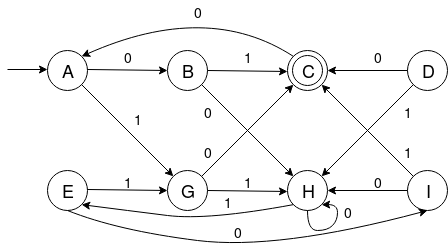
\includegraphics[width=0.5\textwidth]{Slike/autom1.png}
\caption{\label{fig:slika1}Automat sa ekvivalentnim stanjima}
\end{figure}

\noindent Posmatramo A i H. Niska $\epsilon$ ih ne razlikuje jer su oba nezavršna stanja. Niska 0 ih takođe ne razlikuje, jer je $\delta^{*}(A, 0) = B$, a $\delta(H, 0) = H$, gde su $B, H$ oba nezavršna stanja. Isto važi i za nisku 1: $\delta^{*}(A, 1) = G$, $\delta^{*}(H, 1) = E$, gde pritom $G, E \notin F$. Sa druge strane, niska 01 ih razlikuje: $\delta^{*}(A, 01) = C$ i $\delta^{*}(H, 01) = E$, gde C jeste završno stanje, a E nije. \\
Sa druge strane, ako pogledamo A i E, primećujemo da $\delta^{*}(A, 1) = \delta^{*}(E, 1) = G$, što znači da nijedna niska koja počinje sa 1 ne može da ih razlikuje. Niska 0 ih ne razlikuje jer $\delta^{*}(A, 0) = B$, a $\delta^{*}(E, 0) = I$, gde ni $I$ ni $B$ nisu završna stanja. Ako proširimo nisku 0, primećujemo da $\delta^{*}(A, 01) = \delta^{*}(E, 01) = C$ i $\delta^{*}(A, 00) = \delta^{*}(E, 00) = H$, iz čega zaključujemo da su ova dva stanja ekvivalentna. \par


\section{Hopkroftov algoritam}

Hopkroftov algoritam se zasniva na nalaženju količničkog automata za dati DKA, odnosno na određivanju klasa ekvivalencije Nerodove relacije. \par
Ideja algoritma je da se inicijalno stanja podele u dva skupa trivijalno razlikujućih stanja: $S \setminus F$ i $F$, koji su respektivno skupovi nezavršnih i završnih stanja. Glavni korak je tzv. „sečenje particija”. Pretpostavimo da imamo dve particije $Z$ i $Y$, kao i karakter $a$. Kažemo da $Z$ seče $Y$ po karakteru $a$ ukoliko u $Y$ postoji: 
\begin{itemize}
\item bar jedno stanje $y$ za koje $\delta(y, a) \in Z$,
\item bar jedno stanje $y'$ za koje $\delta(y', a) \notin Z$
\end{itemize}
Sečenje particija bi u ovom slučaju predstavljalo podelu particije $Y$ na dva dela:
\begin{itemize}
\item $Y_{1} = \{ y \in Y \ | \ \delta(y, a) \in Z \}$ 
\item $Y_{2} = \{ y \in Y \ | \ \delta(y', a) \notin Z \}$ 
\end{itemize}
Razume se da je sečenje particija ništa drugo do razbijanje postojeće klase ekvivalencije na finije i egzaktnije, to jest odvajanje razlikujućih stanja u zasebne skupove. Algoritam se zaustavlja u trenutku kada ne postoji nijedna particija koja seče neku drugu particiju (ili samu sebe) po nekom slovu, što suštinski znači da jesmo došli do količničkog skupa datog automata. \par
U nastavku sledi pseudo-kod\cite{wiki} Hopkroftovog algoritma.

\vspace{10pt}

\begin{lstlisting}
Algoritam Hopkroft
---------------------------
P := {F, Q \ F};
W := {F};
while (W is not empty) do:
	remove random element A from W;
		for each c in $\Sigma$ do:
			let X be the set of states for which a transition on c leads to a state in A;
			for each set Y in P for which X $\cap$ Y is nonempty and Y \ X is nonempty do:
				replace Y in P by the two sets X $\cap$ Y and Y \ X;
				if Y is in W then:
					replace Y in W by the same two sets;
				else:
					if |X $\cap$ Y| $\leq$ |Y \ X| then:
						add X $\cap$ Y to W;
					else:
						add Y \ X to W;
			end;
		end;
end;
\end{lstlisting}

$P$ predstavlja skup do sada obrađenih particija, a $W$ skup „za obradu”, to jest u skupu $W$ se nalaze sve particije za koje u narednim koracima proveravamo da li seku neku drugu. \par
Algoritam se izvršava u $O(|\Sigma| \ n \ log \ n)$ vremenu, gde je $n$ broj stanja ulaznog automata. Ako pretpostavimo da je kardinalnost azbuke $\Sigma$ konstanta, dolazimo do složenosti $O(n \ log \ n)$.

\vspace{10pt}
\noindent \textbf{Primer 1:}
Posmatrajmo sliku ~\ref{fig:slika1}:
\begin{enumerate}
\item Počinjemo sa $P = \{(C), (A, B, D, E, G, H, I)\}$ i $W = \{(C)\}$, kako je $C$ jedino završno stanje.
\item Uklanjamo element $A$ iz $W$ tako da je $W = \{\}$ i $A = (C)$.
\item Za $c = 0$ formiramo $X_{0} = (G, D)$ i proveravamo $|X_{0} \cap Y \in P|$, kao i $| Y \in P \setminus X_{0}|$.
\item Jasno je da je $X_{0} \cap (C)$ prazan skup, tako da particija (C) ne ispunjava zadati uslov.
\item Kako ga particija $Y = (A, B, D, E, G, H, I) \in P$ ispunjava, delimo je na dva podskupa: $X_{0} \cap Y = (G, D)$ i $Y \setminus X_{0} = (A, B, E, H, I)$ i njih ubacujemo u $P$ umesto originalne particije: \\ $P = \{(C), (G, D), (A, B, E, H, I)\}$.
\item Ubacujemo skup $X_{0} \cap Y$ u $W$, znači sada je $W = \{(G, D)\}$.
\item Za $c = 1$ formiramo $X_{1} = (B, I)$ i proveravamo $|X_{1} \cap Y \in P|$, kao i $| Y \in P \setminus X_{1}|$.
\item Na prvi pogled se vidi da $X_{1}$ seče jedino particiju $Y = (A, B, E, H, I)$, koju dalje delimo na $X_{1} \cap Y = (B, I)$ i $Y \setminus X_{1} = (A, E, H)$ i ubacujemo ih u $P$ umesto originalne particije: \\ $P = \{(C), (G, D), (B, I), (A, E, H)\}$.
\item Ubacujemo skup $X_{0} \cap Y$ u $W$, znači sada je $W = \{(G, D), (B, I)\}$.
\item Uklanjamo element $A$ iz $W$ tako da je $W = \{(B, I)\}$ i $A = (G, D)$.
\item Za $c = 0$ formiramo $X_{0} = ()$, i kako ne postoje stanja koja preko $0$ dolaze do stanja iz $A$, $X_{0}$ je prazno, tako da se algoritam nastavlja dalje jer sečenja particija neće biti.
\item Za $c = 1$ formiramo $X_{1} = (A, E)$ i proveravamo $|X_{1} \cap Y \in P|$, kao i $| Y \in P \setminus X_{1}|$.
\item Vidimo da $X_{1} = (A, E)$ seče particiju $Y = (A, E, H)$, tako da je sada $P = \{(C), (G, D), (B, I), (A, E), (H)\}$.
\item $W = \{(B, I), (H)\}$
\item Uklanjamo element $A$ iz $W$ tako da je $W = \{(H)\}$ i $A = (B, I)$.
\item Za $c = 0$ formiramo $X_{0} = (A, E)$, i kako $X_{0}$ ne seče nijednu particiju, algoritam se nastavlja.
\item Za $c = 1$ formiramo $X_{1} = ()$, i kako ne postoje stanja koja preko $1$ dolaze do stanja iz $A$, $X_{0}$ je prazno, tako da se algoritam nastavlja dalje jer sečenja particija neće biti.
\item Uklanjamo element $A$ iz $W$ tako da je $W = \{\}$ i $A = (H)$.
\item Formiramo $X_{0} = (H, B, I)$ i $X_{1} = (G, D)$, primećujemo da ne seku nijednu particiju i nastavljamo algoritam.
\item Kako je $W = \{\}$, algoritam se završava.
\end{enumerate}

Zaista, dobijene klase ekvivalencije predstavljaju stanja minimalnog DKA~\ref{fig:slika2} za dat početni automat:

\begin{figure}[H]
\centering
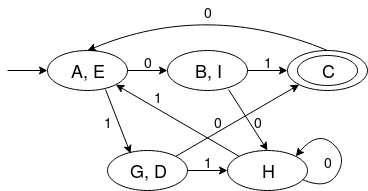
\includegraphics[width=0.6\textwidth]{Slike/autom2.png}
\caption{\label{fig:slika2}Minimalni DKA}
\end{figure}

\newpage

\noindent \textbf{Primer 2:}
Posmatrajmo sliku ~\ref{fig:slika3}:

\begin{figure}[H]
\centering
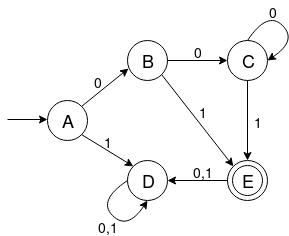
\includegraphics[width=0.4\textwidth]{Slike/autom3.png}
\caption{\label{fig:slika3}Automat sa ekvivalentnim stanjima}
\end{figure}


\begin{enumerate}
\item $P = \{(E), (A, B, C, D)\}$ i $W = \{(E)\}$.
\item $W = \{\}$ i $A = (E)$.
\item $c = 0$, $X_{0} = ()$.
\item $c = 1$, $X_{1} = (B, C)$, $Y = (A, B, C, D)$, $X_{1} \cap Y = (B, C)$, $Y \setminus X_{1} = (A, D)$.
\item $P = \{(E), (A, D), (B, C)\}$, $W = \{(B, C)\}$.
\item $W = \{\}$ i $A = (B, C)$
\item $c = 0$, $X_{0} = (A, B, C)$, $Y = (A, D)$, $X_{0} \cap Y = (A)$, $Y \setminus X_{0} = (D)$.
\item $P = \{(E), (A), (D), (B, C)\}$, $W = \{(A)\}$.
\item $c = 1$, $X_{1} = ()$.
\item $W = \{\}$ i $A = (A)$.
\item $c = 0$, $X_{0} = ()$.
\item $c = 1$, $X_{1} = ()$.
\item $W = \{\}$.
\end{enumerate}

Dobijeni minimalni automat ~\ref{fig:slika4}: 

\begin{figure}[H]
\centering
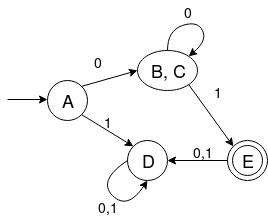
\includegraphics[width=0.4\textwidth]{Slike/autom4.png}
\caption{\label{fig:slika4}Minimalni DKA}
\end{figure}

\newpage

\noindent \textbf{Primer 3:}
Posmatrajmo sliku ~\ref{fig:slika5}:

\begin{figure}[H]
\centering
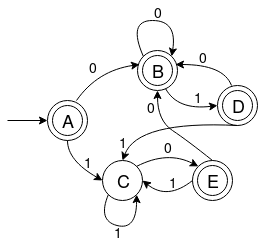
\includegraphics[width=0.35\textwidth]{Slike/autom5.png}
\caption{\label{fig:slika5}Automat sa ekvivalentnim stanjima}
\end{figure}

\begin{enumerate}
\item $P = \{(C), (A, B, D, E)\}$ i $W = \{(C)\}$.
\item $W = \{\}$ i $A = (C)$.
\item $c = 0$, $X_{0} = ()$.
\item $c = 1$, $X_{1} = (A, D, C, E)$, $Y = (A, B, D, E)$, $X_{1} \cap Y = (A, D, E)$, $Y \setminus X_{1} = (B)$.
\item $P = \{(C), (A, D, E), (B)\}$, $W = \{(B)\}$.
\item $W = \{\}$ i $A = (B)$
\item $c = 0$, $X_{0} = (A, B, D, E)$
\item $c = 1$, $X_{1} = ()$.
\item $W = \{\}$
\end{enumerate}

Dobijeni minimalni automat ~\ref{fig:slika6}:
\begin{figure}[H]
\centering
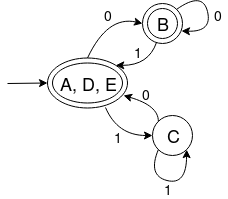
\includegraphics[width=0.35\textwidth]{Slike/autom6.png}
\caption{\label{fig:slika6}Minimalni DKA}
\end{figure}

\section{Zaključak}
U prvom delu ovog rada smo se upoznali sa glavnim pojmovima i terminima potrebnim za razumevanje algoritma. \\
U drugom delu predstavili smo glavnu ideju Hopkroftovog algoritma koji se pokazao kao jako efikasan u praksi.
Uprkos tome što je znatno napredniji od ostalih poznatih algoritama, često biva izostavljen iz literature i gradiva, ili biva pomenut samo u kratkim crtama.  \\
U trećem delu smo naveli nekoliko primera koji bi čitaocu pomogli da intuitivno shvati kako algoritam radi.

\newpage

\begin{thebibliography}{9}

\bibitem{dragonbook06}
  Alfred V. Aho,
  Monica S. Lam,
  Ravi Sethi,
  Jeffrey D. Ullman,
  \textit{Compilers: principles, techniques, \& tools},
  Addison Wesley,
  2nd edition,
  2006.

\bibitem{intro13}
  John E. Hopcroft,
  Rajeev Motwani,
  Jeffrey D. Ullman,
  \textit{Introduction to automata theory, languages, and computation},
  Pearson,
  3rd edition,
  2013.
  
\bibitem{pract17}
  Erin van der Veen,
  \textit{The practical performance of automata minimization algorithms},
  Radboud University,
  Nijmegen, Netherlands,
  2017.
  
\bibitem{hopcroft08}
  Jean Berstel,
  Luc Boasson,
  Olivier Carton,
  \textit{Hopcroft's automaton minimization algorithm and Sturmian words},
  Kiel, Germany,
  2008.
  
\bibitem{hopcrofts11}
  G. Castiglione,
  A. Restivo,
  M. Sciortino,
  \textit{Hopcroft's algorithm and tree-like automata},
  2010.
  
\bibitem{redescribe97}
  Timo Knuutila
  \textit{Re-describing an algorithm by Hopcroft},
  Department of Computer Science,
  University of Turku,
  Turku, Finland,
  1997.
  
\bibitem{onthehopcrofts}
  Andrei P\v aun,
  \textit{On the Hopcroft's minimization algorithm},
  University of Bucharest,
  Bucharest, Romania,
  2007.
  
\bibitem{automatatheory17}
  Javier Esparza,
  \textit{Automata theory: an algorithmic approach, lecture notes},
  2017.
  
\bibitem{around}
  Manuel Baclet,
  Claire Pagetti,
  \textit{Around Hopcroft's algorithm},
  Toulouse, France
  
\bibitem{describing}
  Yingjie XU,
  \textit{Describing an $n log n$ algorithm for minimizing states in deterministic finite automaton},
  2009.
  
\bibitem{wiki}
  Wikipedia article,
  \textit{DFA minimization},
  \href{https://en.wikipedia.org/wiki/DFA_minimization}{link}

\bibitem{ajzenhamer15}
  Nikola Ajzenhamer, 
  Anja Bukurov,
  \textit{Prevođenje programskih jezika: beleške sa predavanja},
  Beograd, Srbija,
  2015.

\end{thebibliography}


\end{document}